\documentclass{article}

\usepackage[preprint,nonatbib]{neurips_2024}

\usepackage[utf8]{inputenc}
\usepackage[T1]{fontenc}
\usepackage{hyperref}
\usepackage{url}
\usepackage{booktabs}
\usepackage{amsfonts}
\usepackage{amsmath}
\usepackage{nicefrac}
\usepackage{microtype}
\usepackage{graphicx}
\usepackage{subcaption}

\hypersetup{colorlinks=true, linkcolor=blue, citecolor=blue, urlcolor=blue}

\title{When Does a Tiny Recursive Proposer Help an Exact\\
Solver? An Inductive, Verifier-Gated Study on\\
Constraint Rostering}

\author{%
  Niraj Pankhania \\
  Coforge \\
  \texttt{niraj.pankhania@coforge.com} \\
}

\begin{document}

\maketitle

\begin{abstract}
Tiny Recursive Models (TRM)~\cite{trm} and their relatives (HRM~\cite{hrm},
PTRM~\cite{ptrm}) reach strong puzzle-solving accuracy with sub-10M-parameter
networks by recursing a small core over an answer state $y$ and a latent state
$z$. Public demonstrations are confined to puzzles and are transductive (a
per-instance identity embedding is learned), which limits transfer to production
constraint problems. We study an inductive, identity-free variant on constraint
rostering---a fixed-size assignment problem with cheaply checkable hard
constraints---under a deliberately constrained CPU-only training budget. We ask a
narrow question: when does a tiny recursive proposer, selected by a deterministic
verifier and backed by an exact CP-SAT fallback, actually reduce solver load, and
when does it not? On a single well-trained configuration we reproduce the TRM
ablation (recursion with deep supervision adds $+23$ points over an equal-parameter
one-pass control on rostering) and find that verifier-gated best-of-$K$ selection
tracks the pass@$K$ oracle (to $91.5\%$) while the learned Q-head plateaus near
$82\%$. A five-seed study at a cheaper budget shows the proposer is high variance
($48\pm8\%$ single-shot valid) but that the verifier-gated hybrid is feasible on
$100\%$ of instances in every seed, degrades gracefully under distribution shift
(feasibility stays $100\%$ as instances get harder), and avoids the exact solver
on the majority of easy instances. The central negative result: the realised
end-to-end speedup \emph{falls} with problem size ($1.9\times \to 1.1\times \to
0.9\times$ at $30/48/70$ cells) because proposer accuracy collapses faster than
CP-SAT slows at these (solver-easy) scales. An off-the-shelf 0.5B language model,
few-shot, produces no feasible rosters. We conclude the verifier-plus-fallback
construction is sound and a useful safety wrapper, but that its economic value is
conditional on regimes where the exact solver is expensive---which these instance
sizes are not.
\end{abstract}

\section{Introduction}

Recursive-reasoning models challenge the premise that strong reasoning requires
scale. HRM~\cite{hrm} couples two recurrent modules at different timescales; TRM
\cite{trm} reduces this to a single two-layer network recursed over an answer
state $y$ and a latent state $z$ with deep supervision and weight EMA, and reports
$45\%$ on ARC-AGI-1 with $7$M parameters; PTRM~\cite{ptrm} adds test-time
stochasticity (per-step Gaussian noise, $K$ parallel rollouts, Q-head selection).
These results are reported on abstract puzzles, and the training setups are
transductive: each instance carries a learned identity embedding, so the model
answers only instances seen in training.

Two gaps follow. First, it is unknown whether the recursion mechanism transfers,
inductively, to a constrained industrial problem with a real cost model. Second,
the literature recommends deploying such a model as a cheap proposer behind an
exact solver, but the economics of that pattern have not been measured. We address
both on constraint rostering---assigning workers to shifts subject to coverage,
rest, and workload rules---chosen because it is a fixed-size assignment problem
with a cheap, sound feasibility check and an off-the-shelf exact solver (CP-SAT).

We do not propose a new architecture; our contributions are empirical.
\begin{enumerate}
\item An inductive (identity-free) instantiation of a TRM-style model on a
non-puzzle constraint task, evaluated on held-out instances
(Section~\ref{sec:method}).
\item A controlled comparison of verifier-gated best-of-$K$ selection against the
learned Q-head and majority voting, quantifying the selection gap
(Section~\ref{sec:selection}).
\item A multi-seed robustness, generalization, and cost study of the
proposer-plus-exact-solver hybrid, including a negative result on how realised
speedup scales with problem size (Section~\ref{sec:pilot}).
\end{enumerate}
We report results under two training budgets and are explicit about which claims
rest on a single seed versus five seeds.

\section{Related Work}

\paragraph{Recursive reasoning.} TRM~\cite{trm} and HRM~\cite{hrm} established the
tiny-recursion paradigm on Sudoku, Maze and ARC. PTRM~\cite{ptrm} is the closest
methodological antecedent for our inference procedure: it injects per-step
Gaussian noise ($\sigma$) and selects the best of $K$ rollouts with the model's
Q-head. We adopt PTRM-style noise but replace Q-head selection with a
deterministic verifier and add an exact-solver fallback.

\paragraph{Learning-augmented rostering.} \cite{dnnts} (DNNTS) train a DNN to guide
branch-and-bound for personnel rostering; \cite{nurserepair} use a DNN to repair
MIP-generated nurse schedules toward hidden acceptability constraints. Closest to
our setting, \cite{patat} train a transformer on CP-generated feasible nurse
schedules and probe learnability, reporting a hierarchy (local per-nurse rules are
learned; global cross-nurse rules are not) and proposing the outputs as warm
starts for repair. None of these is a recursive reasoning model, and none couples
verifier-gated test-time scaling with an exact-solver fallback. Our position is
narrow: a tiny recursive proposer, trained inductively, wrapped so that every
returned solution is verifier-passed or solver-exact, with the hybrid's economics
measured against the solver it is meant to offload.

\section{Method}
\label{sec:method}

\paragraph{Model.} A single core is a 2-layer MLP-mixer~\cite{mlpmixer}
(token-mixing plus channel-mixing SwiGLU), recursed over two states: the answer
logits $y$ and a latent $z$. One recursion \emph{block} performs $n$ latent updates
$z \leftarrow \mathrm{core}(x_e, y, z)$ followed by one answer update
$y \leftarrow \mathrm{core}(x_e, y, z)$, where $x_e$ is the token embedding of the
partial assignment. Deep recursion applies $T$ blocks with gradient restricted to
the last block (truncated BPTT); deep supervision applies the loss at each of
$N_{\mathrm{sup}}$ outer steps with a detached carry. We keep a weight EMA and a
Q/halt head trained with a binary correctness target. The loss per supervision
step is masked cross-entropy over \emph{blank} cells only plus a Q-head BCE term:
$\mathcal{L} = \mathrm{CE}_{\mathrm{mask}}(f_O(y), y^\star) + \lambda\,
\mathrm{BCE}(\hat q, \mathbf{1}[\hat y = y^\star])$, $\lambda = 0.5$. Masking is
necessary: supervising given cells lets the model copy inputs and collapses
blank-cell accuracy.

\paragraph{Inductive conditioning.} Unlike TRM/HRM/PTRM we use no per-instance
identity embedding; inputs are token and positional embeddings only. The model
therefore learns general constraint structure and is tested on instances it never
saw.

\paragraph{Verifier-gated inference.} Following PTRM we add Gaussian noise
$z \leftarrow z + \sigma\,\varepsilon$ at each recursion step and run $K$ parallel
rollouts. We select the output using the problem's deterministic feasibility
checker rather than the Q-head. We compare four selectors: pass@$K$ (oracle, any
rollout correct), verifier@$K$ (first verifier-passing rollout), Q-head best@$K$,
and majority@$K$.

\paragraph{Hybrid with exact fallback.} At deployment the proposer runs $K$
verifier-gated rollouts; if none passes, control falls back to an exact CP-SAT
solve~\cite{ortools}. Every returned solution is thus verifier-passed or
solver-exact, so the proposer can only change cost, never feasibility.

\paragraph{Data and label consistency.} Instances are generated by CP-SAT; a
partial assignment is produced by blanking cells of a full solution. Supervised
per-cell training requires a unique label, so we filter training and test
instances to those with a \emph{unique} completion (verified by CP-SAT solution
counting, cutting off at two solutions). On the unfiltered many-completion
distribution the model collapses ($\sim$2\% valid): per-cell supervision cannot fit
a one-to-many map. This is a real limitation, not a tuning artefact.

\section{Experimental Setup}

\paragraph{Tasks.} (i) $4\times4$ Sudoku, 8 of 16 cells blanked, as a validated CSP
control. (ii) Shift rostering on a $W\times D$ grid: each day needs exactly
$\lfloor W/3\rfloor$ day and $1$ night shift, no night-then-day transition, and at
most $D{-}1$ shifts per worker; cells are OFF/DAY/NIGHT. The primary grid is
$6\times5$ ($30$ cells); scaling uses $8\times6$ ($48$) and $10\times7$ ($70$).

\paragraph{Model and optimisation.} Core hidden width $128$, $2$ layers,
$n{=}4$ latent updates, $T{=}2$ blocks, $N_{\mathrm{sup}}{=}4$; $\sim$228K
parameters. The one-pass control sets $n{=}0, T{=}1, N_{\mathrm{sup}}{=}1$ with the
\emph{same} architecture and parameter count. Training: AdamW
($\mathrm{lr}=3\!\times\!10^{-3}$, weight decay $0.1$, $\beta=(0.9,0.95)$), cosine
schedule, gradient clip $1.0$, batch $512$, EMA decay $0.995$; evaluation uses the
EMA weights. All runs are CPU-only (Apple silicon, $4$ threads). Inference uses
$\sigma{=}0.5$ (rostering) / $0.4$ (Sudoku) and $K\in\{1,4,16,64\}$; the hybrid
uses $K{=}16$.

\paragraph{Two budgets.} We report two configurations explicitly.
\emph{Budget~A (single seed, well-trained):} $1400$ training instances (Sudoku
$2000$), $\sim$175 epochs, used for the ablation and the selection study
(Sections~\ref{sec:ablation}--\ref{sec:selection}). \emph{Budget~B (five seeds,
strictly time-budgeted, $<$10\,min/run):} $1000$ training instances, $90$--$165$
epochs, used for all robustness, generalization, and economic claims
(Section~\ref{sec:pilot}). The gap between the two (below) is itself evidence of
seed/budget sensitivity, and we treat Budget-A numbers as indicative.

\section{Results}

\subsection{Recursion vs.\ one pass at equal parameters (Budget A, single seed)}
\label{sec:ablation}

\begin{table}[h]
\centering
\caption{Recursion with deep supervision vs.\ an equal-parameter one-pass control
($\sim$228K params). Single seed.}
\label{tab:ablation}
\begin{tabular}{lccc}
\toprule
Task & One-pass & Recursive & $\Delta$ \\
\midrule
Sudoku $4\times4$ (8 blanks) & 81.0\% & 99.5\% & $+18.5$ \\
Rostering $6\times5$ (6 blanks) & 58.5\% & 81.5\% & $+23.0$ \\
\bottomrule
\end{tabular}
\end{table}

With architecture and parameter count held fixed, recursion with deep supervision
adds $18$--$23$ points (Table~\ref{tab:ablation}, Figure~\ref{fig:ablation}),
consistent with the central TRM claim that the gain is from iterative refinement
rather than capacity. As a single-seed result we treat the magnitude as indicative;
Budget-B below shows the recursive model's absolute accuracy is seed- and
budget-sensitive.

\begin{figure}[h]
\centering
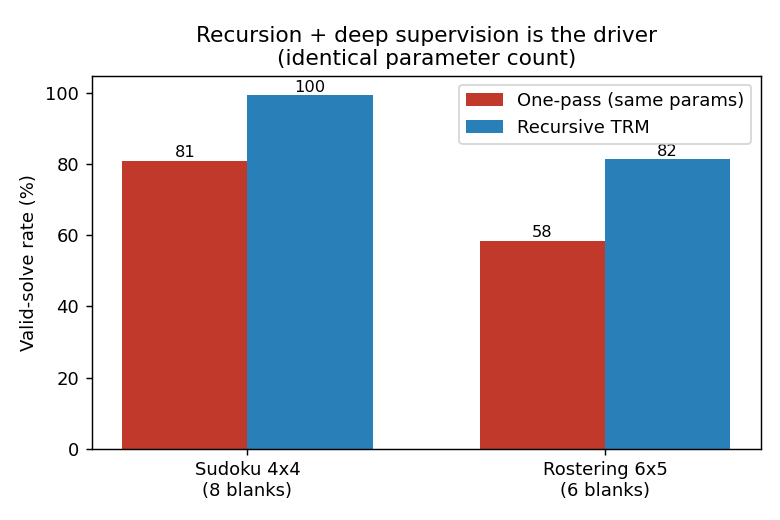
\includegraphics[width=0.5\textwidth]{figs/ablation.png}
\caption{Recursion vs.\ one pass at equal parameters (Budget A).}
\label{fig:ablation}
\end{figure}

\subsection{Selection: verifier vs.\ Q-head vs.\ majority (Budget A, single seed)}
\label{sec:selection}

\begin{table}[h]
\centering
\caption{Rostering $6\times5$ test-time scaling (\% feasible). Verifier tracks the
pass@$K$ oracle; the Q-head does not.}
\label{tab:selection}
\begin{tabular}{lccccc}
\toprule
$K$ & 1 & 4 & 16 & 32 & 64 \\
\midrule
pass@$K$ (oracle) & 81.0 & 87.5 & 90.0 & 91.0 & 91.5 \\
verifier@$K$ & 81.0 & 87.5 & 90.0 & 91.0 & 91.5 \\
Q-head best@$K$ & 81.0 & 81.5 & 82.0 & 79.5 & 79.5 \\
majority@$K$ & 81.0 & 82.5 & 82.0 & 82.0 & 82.0 \\
\bottomrule
\end{tabular}
\end{table}

A sound verifier recovers the pass@$K$ oracle exactly (both reach $91.5\%$ at
$K{=}64$), whereas Q-head and majority selection plateau near $82\%$
(Table~\ref{tab:selection}, Figure~\ref{fig:scaling}). For constraint problems,
which provide a verifier for free, learned-ranking selection is strictly
dominated; we use the verifier throughout.

\begin{figure}[h]
\centering
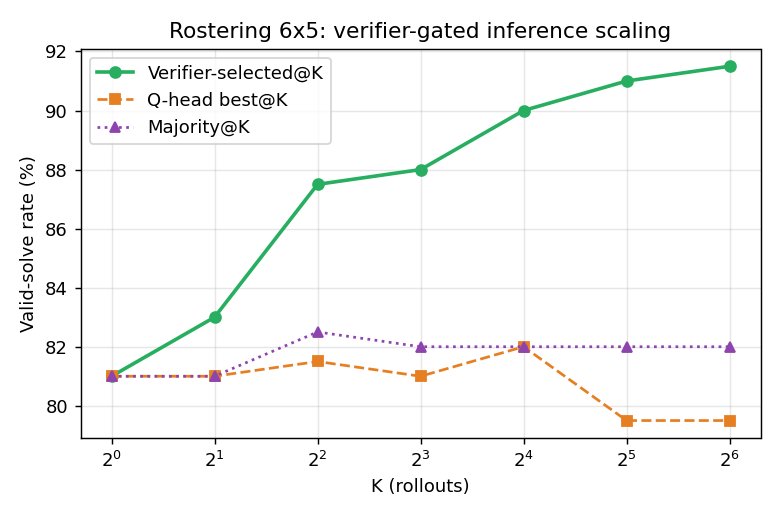
\includegraphics[width=0.5\textwidth]{figs/scaling_roster.png}
\caption{Rostering test-time scaling (Budget A): verifier tracks the oracle, the
Q-head plateaus.}
\label{fig:scaling}
\end{figure}

\subsection{Robustness, generalization, and economics (Budget B, five seeds)}
\label{sec:pilot}

\paragraph{Variance.} Across five seeds on $6\times5$, single-shot valid rate is
$48\pm8\%$ and verifier@16 is $59\pm7\%$ (population std). Hybrid feasibility is
$100\%$ in \emph{every} seed (Figure~\ref{fig:pilot}a). The spread confirms that
single-seed accuracy figures---including Budget A's $81.5\%$---should not be read as
point estimates; absolute accuracy is sensitive to seed and training budget, while
the hybrid's feasibility guarantee is not.

\paragraph{Distribution shift.} Training at 6 blanks and testing at 6/8/10,
verifier@16 falls $60\%\to42\%\to34\%$ (3-seed mean), while hybrid feasibility
stays $100\%$ throughout: the proposer's hit-rate degrades, but correctness does
not, because out-of-distribution instances route to the exact solver.

\paragraph{Economics vs.\ size.} Per attempt the proposer is $\sim$7--8$\times$
cheaper than a CP-SAT solve at all sizes, but the realised end-to-end speedup
falls with size (Table~\ref{tab:econ}, Figure~\ref{fig:pilot}b): as the grid grows
under a fixed cheap budget, proposer accuracy collapses ($48\%\to28\%\to2\%$)
faster than CP-SAT slows, so more instances hit the fallback and at $70$ cells the
hybrid is slower than calling the solver directly. At these sizes CP-SAT is itself
sub-millisecond, so there is little to offload; the pattern pays off only where the
exact solver is expensive.

\begin{table}[h]
\centering
\caption{Cost vs.\ size (Budget B). Per-instance times in ms; speedup is
hybrid vs.\ solver-only.}
\label{tab:econ}
\begin{tabular}{lccccc}
\toprule
Size & Cells & Proposer valid & CP-SAT ms & TRM ms & Realised speedup \\
\midrule
$6\times5$ & 30 & 48\% & 0.82 & 0.10 & $1.9\times$ \\
$8\times6$ & 48 & 28\% & 0.93 & 0.14 & $1.1\times$ \\
$10\times7$ & 70 & \phantom{0}2\% & 1.23 & 0.16 & $0.9\times$ \\
\bottomrule
\end{tabular}
\end{table}

\paragraph{Off-the-shelf SLM baseline.} On $6\times5$, Qwen2.5-0.5B-Instruct
\cite{qwen} prompted few-shot ($n{=}50$, no fine-tuning) produced $0\%$ feasible
rosters (52\% of outputs even parsed to a complete grid) at $3.3$\,s/instance:
$>$2000$\times$ the proposer's parameters and $\sim$30{,}000$\times$ its per-attempt
latency (Figure~\ref{fig:pilot}c). This bounds the zero-shot capability of a
general small LM on the task; a fine-tuned SLM would be a stronger, fairer
comparator and is left to future work.

\begin{figure}[h]
\centering
\begin{subfigure}{0.32\textwidth}
  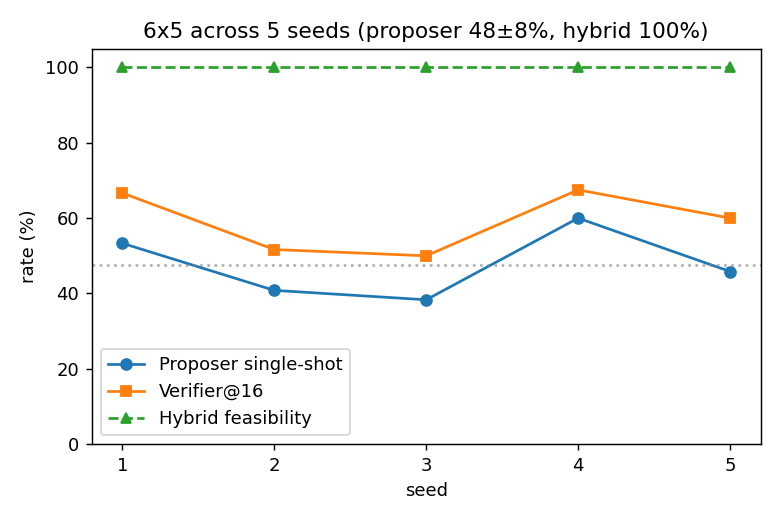
\includegraphics[width=\linewidth]{figs/ws1_seeds.png}
  \caption{Five seeds, $6\times5$.}
\end{subfigure}\hfill
\begin{subfigure}{0.32\textwidth}
  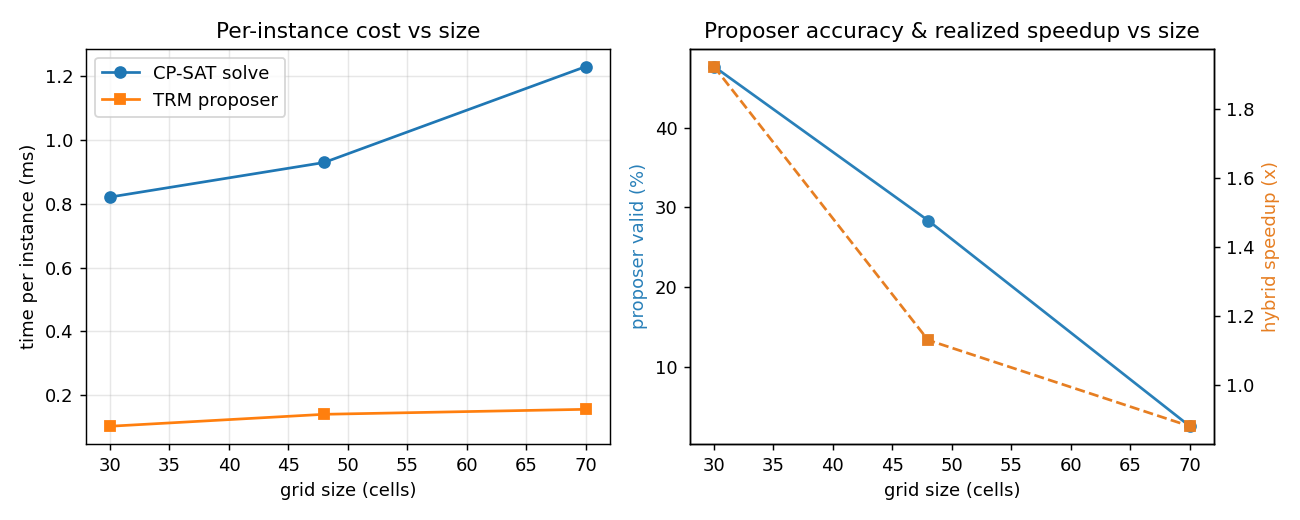
\includegraphics[width=\linewidth]{figs/ws3_size.png}
  \caption{Cost and speedup vs.\ size.}
\end{subfigure}\hfill
\begin{subfigure}{0.32\textwidth}
  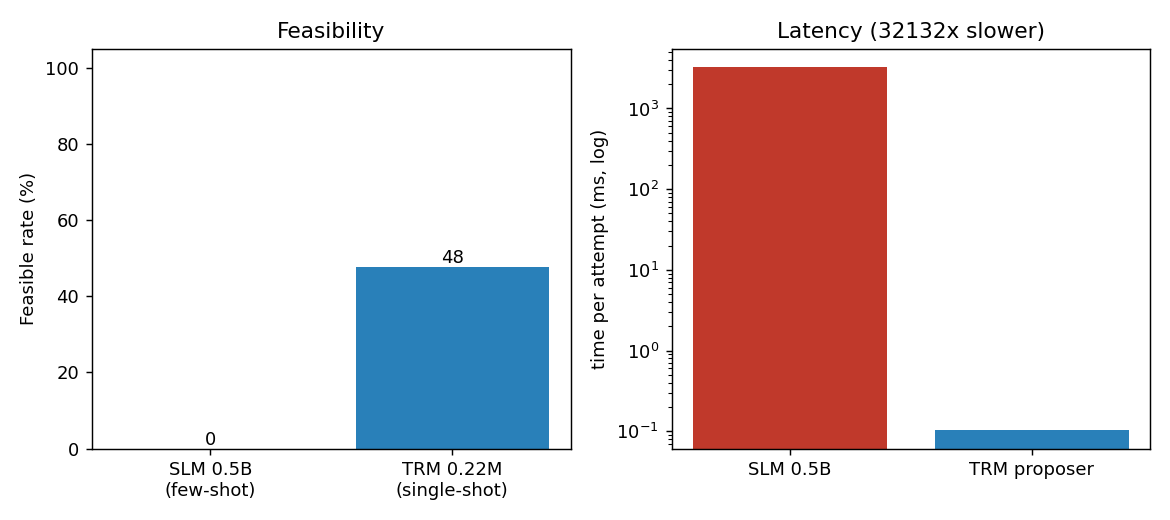
\includegraphics[width=\linewidth]{figs/ws4_slm.png}
  \caption{SLM vs.\ proposer.}
\end{subfigure}
\caption{Budget-B study. (a) Hybrid feasibility is $100\%$ on all seeds despite
proposer variance. (b) Per-attempt the proposer is cheaper, but realised speedup
falls with size and drops below $1\times$ at $70$ cells. (c) A $0.5$B SLM is $0\%$
feasible and orders of magnitude slower.}
\label{fig:pilot}
\end{figure}

\section{Discussion and Threats to Validity}

The verifier-plus-fallback construction behaves as designed: it is sound by
construction and fails safe under shift, and selection by a deterministic verifier
strictly dominates the learned Q-head. The useful regime is narrow and
identifiable: fixed-size problems with a cheap sound check where the exact solver
is the bottleneck. Our instances do not meet the last condition---CP-SAT is
sub-millisecond---so the economic case is not demonstrated here and, at $70$ cells,
is negative. Transfer to regimes where it would matter (larger, solver-expensive
instances; soft-objective optimisation rather than feasibility) is untested.

Threats to validity we are aware of: (1) the ablation and selection results are
single-seed (Budget A) and the large gap to Budget B shows accuracy is
budget/seed-sensitive; (2) absolute accuracy is low under the cheap budget by
design; (3) the SLM baseline is zero/few-shot, not fine-tuned; (4) unique-
completion filtering restricts the training distribution and is required for
supervised per-cell learning; (5) all problems are synthetic and small.

\section{Conclusion}

An inductive, tiny recursive proposer with verifier-gated selection and an exact-
solver fallback reproduces the recursion-is-the-driver result, recovers the
pass@$K$ oracle via a verifier where the learned Q-head cannot, and guarantees
feasibility under distribution shift. Its economic value, however, is conditional:
under a cheap training budget the realised speedup falls with size and turns
negative once per-instance solver time is sub-millisecond. The construction is a
sound safety wrapper; establishing its economic value requires regimes where the
exact solver is expensive, multi-seed training at each size, and a fine-tuned
small-LM comparator---the targets of future work.

\begin{thebibliography}{9}

\bibitem{trm}
A.~Jolicoeur-Martineau.
\newblock Less is More: Recursive Reasoning with Tiny Networks.
\newblock \emph{arXiv:2510.04871}, 2025.

\bibitem{hrm}
G.~Wang, J.~Li, Y.~Sun, X.~Chen, C.~Liu, Y.~Wu, M.~Lu, S.~Song, and
Y.~Abbasi~Yadkori.
\newblock Hierarchical Reasoning Model.
\newblock \emph{arXiv:2506.21734}, 2025.

\bibitem{ptrm}
Probabilistic Tiny Recursive Model (PTRM).
\newblock \emph{arXiv:2605.19943}, 2026.

\bibitem{dnnts}
Z.~Chen, P.~De~Causmaecker, and Y.~Dou.
\newblock Neural Networked Assisted Tree Search for the Personnel Rostering
Problem.
\newblock \emph{arXiv:2010.14252}, 2020.

\bibitem{nurserepair}
A solution method of nurse scheduling problem using machine learning.
\newblock \emph{Journal of Advanced Mechanical Design, Systems, and
Manufacturing}, 20(5), 2026.

\bibitem{patat}
Constraint Learning and Schedule Proposal via Transformers for the Nurse
Scheduling Problem.
\newblock \emph{Proc.\ PATAT}, 2026.

\bibitem{mlpmixer}
I.~Tolstikhin, N.~Houlsby, A.~Kolesnikov, L.~Beyer, X.~Zhai, T.~Unterthiner,
J.~Yung, A.~Steiner, D.~Keysers, J.~Uszkoreit, M.~Lucic, and A.~Dosovitskiy.
\newblock MLP-Mixer: An all-MLP Architecture for Vision.
\newblock \emph{NeurIPS}, 2021.

\bibitem{ortools}
L.~Perron and F.~Didier.
\newblock OR-Tools CP-SAT Solver.
\newblock Google, 2024. \url{https://developers.google.com/optimization}.

\bibitem{qwen}
Qwen Team.
\newblock Qwen2.5 Technical Report.
\newblock \emph{arXiv:2412.15115}, 2024.

\end{thebibliography}

\end{document}
